%%%%%%%%%%%%%%%%%%%%%%%%%%%%% Define Article %%%%%%%%%%%%%%%%%%%%%%%%%%%%%%%%%%
\documentclass[a4paper]{article}
%%%%%%%%%%%%%%%%%%%%%%%%%%%%%%%%%%%%%%%%%%%%%%%%%%%%%%%%%%%%%%%%%%%%%%%%%%%%%%%

%%%%%%%%%%%%%%%%%%%%%%%%%%%%% Using Packages %%%%%%%%%%%%%%%%%%%%%%%%%%%%%%%%%%
\usepackage[a4paper,top=3cm,bottom=2cm,left=2cm,right=2cm,marginparwidth=1.75cm]{geometry}
\usepackage{graphicx}
\usepackage{amssymb}
\usepackage{amsmath}
\usepackage{amsthm}
\usepackage{empheq}
\usepackage{mdframed}
\usepackage{booktabs}
\usepackage{lipsum}
\usepackage{graphicx}
\usepackage{color}
\usepackage{psfrag}
\usepackage{pgfplots}
\usepackage{bm}
\usepackage[colorinlistoftodos]{todonotes}
\usepackage[colorlinks=true, allcolors=blue]{hyperref}
\usepackage{caption}
\usepackage{subcaption}
\usepackage{sectsty}
\usepackage{apacite}
\usepackage{float}
\usepackage{titling} 
\usepackage{blindtext}
\usepackage[square,sort,comma,numbers]{natbib}
\usepackage[colorinlistoftodos]{todonotes}
\usepackage{xcolor}
\usepackage{listings}
\usepackage{setspace} \doublespacing

\usepackage{color} %red, green, blue, yellow, cyan, magenta, black, white
\definecolor{mygreen}{RGB}{28,172,0} % color values Red, Green, Blue
\definecolor{mylilas}{RGB}{170,55,241}
%%%%%%%%%%%%%%%%%%



\definecolor{darkgreen}{rgb}{0.0, 0.4, 0.0}

%%%%%%%%%Search overleaf site for headers%%%%%%%%%%%%%%%%%%
\usepackage{fancyhdr}
%%%%%%%%%%%%%%%%%%%%%%%%%%%%%%%%%%%%%%%%%%%%%%%%%%%%%%%%%%%%%%%%%%%%%%%%%%%%%%%

% Other Settings

%%%%%%%%%%%%%%%%%%%%%%%%%% Page Setting %%%%%%%%%%%%%%%%%%%%%%%%%%%%%%%%%%%%%%%
\geometry{a4paper}

%%%%%%%%%%%%%%%%%%%%%%%%%% Define some useful colors %%%%%%%%%%%%%%%%%%%%%%%%%%
\definecolor{ocre}{RGB}{243,102,25}
\definecolor{mygray}{RGB}{243,243,244}
\definecolor{deepGreen}{RGB}{26,111,0}
\definecolor{shallowGreen}{RGB}{235,255,255}
\definecolor{deepBlue}{RGB}{61,124,222}
\definecolor{shallowBlue}{RGB}{235,249,255}
%%%%%%%%%%%%%%%%%%%%%%%%%%%%%%%%%%%%%%%%%%%%%%%%%%%%%%%%%%%%%%%%%%%%%%%%%%%%%%%

%%%%%%%%%%%%%%%%%%%%%%%%%% Define an orangebox command %%%%%%%%%%%%%%%%%%%%%%%%
\newcommand\orangebox[1]{\fcolorbox{ocre}{mygray}{\hspace{1em}#1\hspace{1em}}}
%%%%%%%%%%%%%%%%%%%%%%%%%%%%%%%%%%%%%%%%%%%%%%%%%%%%%%%%%%%%%%%%%%%%%%%%%%%%%%%

%%%%%%%%%%%%%%%%%%%%%%%%%%%% English Environments %%%%%%%%%%%%%%%%%%%%%%%%%%%%%
\newtheoremstyle{mytheoremstyle}{3pt}{3pt}{\normalfont}{0cm}{\rmfamily\bfseries}{}{1em}{{\color{black}\thmname{#1}~\thmnumber{#2}}\thmnote{\,--\,#3}}
\newtheoremstyle{myproblemstyle}{3pt}{3pt}{\normalfont}{0cm}{\rmfamily\bfseries}{}{1em}{{\color{black}\thmname{#1}~\thmnumber{#2}}\thmnote{\,--\,#3}}
\theoremstyle{mytheoremstyle}
\newmdtheoremenv[linewidth=1pt,backgroundcolor=shallowGreen,linecolor=deepGreen,leftmargin=0pt,innerleftmargin=20pt,innerrightmargin=20pt,]{theorem}{Theorem}[section]
\theoremstyle{mytheoremstyle}
\newmdtheoremenv[linewidth=1pt,backgroundcolor=shallowBlue,linecolor=deepBlue,leftmargin=0pt,innerleftmargin=20pt,innerrightmargin=20pt,]{definition}{Definition}[section]
\theoremstyle{myproblemstyle}
\newmdtheoremenv[linecolor=black,leftmargin=0pt,innerleftmargin=10pt,innerrightmargin=10pt,]{problem}{Problem}[section]
%%%%%%%%%%%%%%%%%%%%%%%%%%%%%%%%%%%%%%%%%%%%%%%%%%%%%%%%%%%%%%%%%%%%%%%%%%%%%%%

%%%%%%%%%%%%%%%%%%%%%%%%%%%%%%% Plotting Settings %%%%%%%%%%%%%%%%%%%%%%%%%%%%%
\usepgfplotslibrary{colorbrewer}
\pgfplotsset{width=8cm,compat=1.9}
%%%%%%%%%%%%%%%%%%%%%%%%%%%%%%%%%%%%%%%%%%%%%%%%%%%%%%%%%%%%%%%%%%%%%%%%%%%%%%%

%%%%%%%%%%%%%%%%%%%%%%%%%%%%%%% Title & Author %%%%%%%%%%%%%%%%%%%%%%%%%%%%%%%%
\title{Computer Graphics Tehqiq - Final Report}
\author{Muhammad Meesum Ali Qazalbash}
%%%%%%%%%%%%%%%%%%%%%%%%%%%%%%%%%%%%%%%%%%%%%%%%%%%%%%%%%%%%%%%%%%%%%%%%%%%%%%%
\begin{document}

\begin{titlepage}

    \newcommand{\HRule}{\rule{\linewidth}{0.5mm}} 							% horizontal line and its thickness
    \center

    % University
    \textsc{\LARGE Habib University}\\[1cm]

    % Document info
    \textsc{\Large Implementing the Graphics Pipeline}\\[0.2cm]
    \textsc{\large STRP 2022}\\[1cm] 										% Course Code
    \HRule \\[0.8cm]
    { \huge \bfseries Final Research Report}\\[0.7cm]								% Assignment
    \HRule \\[2cm]
    \large
    \emph{Muhammad Meesum Ali Qazalbash}\\
    ID: 06861\\ Supervisor: \emph{Dr Waqar Saleem}\\[1.5cm]													% Author info
    {\large \today}\\[5cm]
    
\includegraphics[width=0.6\textwidth]{HU-LOGO--01.jpg}\\[1cm] 	% University logo
    \vfill

\end{titlepage}
\newpage
\tableofcontents
\newpage
% \maketitle
\section{Problem Statement}
To bring the graphics pipeline into software. The pipeline is tasked with rendering the scene on the screen. The pipeline will serve as a template for students in following CG courses.

\section{Rationale}
Graphical Pipeline is often implemented as hardware on GPUs. We will create the pipeline in software to better understand it. Later on, we'd like students to construct their own pipeline, stage by stage.

\section{Literature Review}

\subsection{Introduction}
This was my first introduction to computer graphics. Dr. Waqar Saleem recomended a book \emph{Interactive Computer Graphics: A Top-Down Approach with WebGL}\cite{book}, 7th edition, for my foundational knowledge. The fundamentals of computer graphics and the elements necessary to comprehend the graphical pipeline were both addressed in this book.

\subsection{Related Work}
I identified a handful repositories on GitHub. They were decent, but virtually all of them either employed any framework or library that ran the pipeline on the GPU, such as WebGL, OpenGL, or DirectX, or their code was very specific to the purpose. Because we want to emulate the pipeline on the CPU, this was not a suitable assistance for our project.

\subsection{WebGL for experiments}
I used WebGL - a framework of JavaScript for computer graphics - to get some hands on experince of how the shader works and likewise how the pipeline works. WebGL was very well developed and was very easy to use. I used basic structure of the WebGL to design my own pipeline.

\newpage

\section{Design \& Methodologies}

The pipeline is inspired from the working of WebGL. There are three major stages in WebGL.
\begin{enumerate}
    \item Application Program
    \item GL Context
    \item Graphical Pipeline
\end{enumerate}

\begin{figure}[h]
    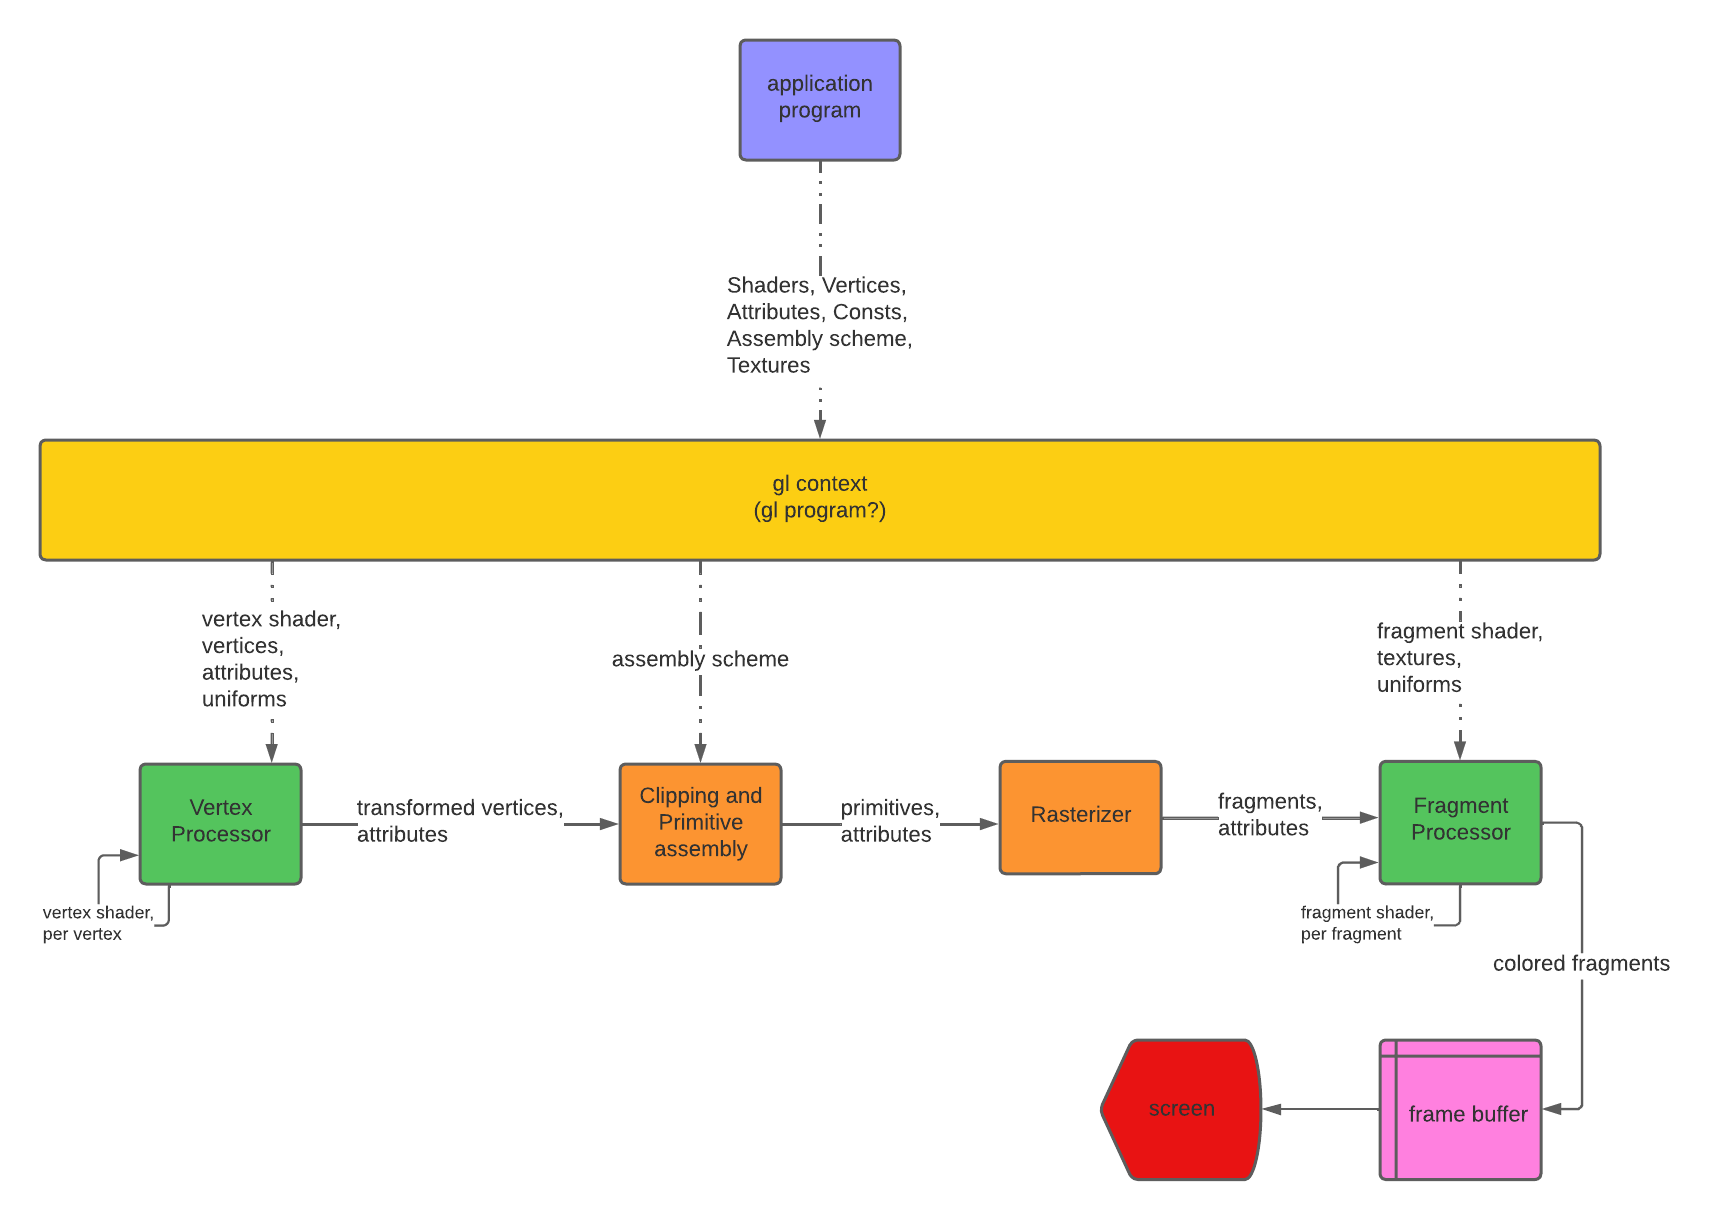
\includegraphics[width=\textwidth]{pipeline-design.png}
    \caption{Design of the pipeline}
    \label{pipeline}
\end{figure}

\subsection{Application Program}
The application program is provided with all the essential pieces of the pipeline.
\subsection{GL Context}
The gl-context is the object that is used to store all the information about the pipeline. This object can be accessed by any stage in the pipeline.

\subsection{Graphical Pipeline}
Then there are four stages in the pipeline. In the \ref{pipeline}, the stages are depicted. Two of them are green and other two are orange. Green stages are programmable, which means that the program that would run on in these stages is provided by the user. Orange stages are fixed, which means that their logic is fixed.

\subsubsection{Vertex Processor}
The only task of the vertex processor is to run the vertex shader. The shader will be provided by the user. But there is one constraint on it is that the shader can only have two parameter; first one is the dictionary with all attributes of the vertex and second one is the dictionary with all uniforms, and the shader should return the transformed vertex as a 4-dimensional vector.

\subsubsection{Clipping \& Primitive Assembly}
The clipping stage would clip and assemble vertices into the primitives. The assembling scheme is provided by the user. There are seven different types of assembling schemes that we have considered.
\begin{enumerate}
    \item Point
    \item Line
    \item Line-strip
    \item Line-loop
    \item Triangle
    \item Triangle-strip
    \item Triangle-fan
\end{enumerate}

This stage will return the vertices that are inside the viewport as primitives.

\subsubsection{Rasterizer}
The rasterizer's task is the most simple of all, it has to raster the primitives coming from the clipping stage. It will return the fragments that are raster by the primitives.

\subsubsection{Fragment Processor}
The fragments coming from the rasterizer are colored in the fragment processor. The fragment processor will run the fragment shader - provided by the user -  to color each fragment. There are same restrictions on fragment shader as of vertex shader. The fragment shader instead of returning colored fragments to frame buffer, it would render the scene as a form of image.

\section{Research Results}
The result is the pipeline soley built on python3 that is running on CPU, but It is a little but faster because of the vecotrization in the Clipping \& Primitive Assembly Stage and Rasterizer Stage. The pipeline is in the \href{https://GitHub.com/ai-maq/Computer-Graphics-Tehqiq/}{GitHub repository}. One of the output from the pipeline is the rendered image.

%will insert the image here%


\section{Conclusion}
We have successfully emulated the graphical pipeline in software, before that it was only existing in the hardware on GPUs.

\section{Reflections on Research Journey}

\section{Acknowledgements}
\begin{thebibliography}{9}
    \bibitem{book}
    Angel, E. and Shreiner, D., 2016. \emph{Interactive Computer Graphics: A Top-Down Approach with WebGL}. 7th ed. Boston [etc.]: Pearson.
\end{thebibliography}

\end{document}